\chapter{Processo de Desenvolvimento}

Conforme as boas práticas que a Engenharia de Software prega, para que um projeto de software obtenha êxito quanto ao cumprimento de seus requisitos, é necessário que este seja desenvolvido de maneira sistemática e organizada. Por isso, processos de desenvolvimento de software são criados para auxiliar esta sistematização, consequentemente agregando valor ao trabalho dos desenvolvedores e ao produto final. Atualmente, organizações regulamentadoras como a ISO \cite{iso}, utilizam como parâmetro de classificação de qualidade a verificação de quais processos de software são empregados nas instituições.

Conhecendo a grande importância que um processo de desenvolvimento exerce sobre a qual\-idade do produto final, buscou-se um processo, dentre os existentes na literatura especializada, que mais se adequasse ao contexto do projeto. Dentre os processos existentes optou-se pela escolha do XP1 \cite{xp1}, os motivos para deste ante os demais processos existentes foram os seguintes: i) trata-se de um processo bastante simplificado e indica a produção de um conjunto limitado de artefatos, logo, não traria maior \textit{overhead} para a equipe de desenvolvedores; ii) trata-se de um processo desenvolvido por um conjunto de alunos e professores da Universidade Federal de Campina (UFCG). Tal fato trouxe a segurança que as possíveis dificuldades que aparecessem poderiam ser facilmente dissipadas pois a equipe de desenvolvimento estaria em contato direto com os autores do processo; iii) este processo tem obtido grandes sucessos no contexto acadêmico; e iv) o processo em si agrupa um conjunto de práticas já bastante utilizadas por empresas e segue as diretrizes principais de um bom processo de desenvolvimento conforme indica a Engenharia de Software.

É importante comentar que o processo XP1 foi escolhido como base para realização do nosso projeto, porém como acontece na maioria das empresas que adotam um processo, foi necessário realizar algumas adaptações do mesmo para melhor refletir o contexto ao qual o projeto, ora descrito, estava inserido.

XP1 define um conjunto de papéis que os membros da equipe deverão assumir no decorrer do desenvolvimento, bem como quais responsabilidades cada pessoa que assumir tal papel terá. Os papéis, bem como as suas respectivas responsabilidades, estão listados a seguir: \\

\textbf{Papel: Cliente}
\begin{itemize}
 \item Descrever a funcionalidade desejada.
 \item Descrever os requisitos não funcionais do software.
 \item Definir o plano de release de software.
 \item Descrever os testes de aceitação para cada \textit{User Story}.
 \item Escolher User Stories para cada iteração.
\end{itemize}

\textbf{Papel: Desenvolvedor}
\begin{itemize}
 \item Ajudar a levantar User Stories e requisitos não funcionais junto ao cliente.
 \item Elaborar um projeto arquitetural.
 \item Estimar o tempo de desenvolvimento de \textit{User Stories} e tarefas.
 \item Elaborar o esquema lógico dos dados.
 \item Escrever o código das tarefas e Testes de Unidade.
 \item Executar atividades de integração e \textit{Test Review}.
 \item Implementar a automação de Testes de Aceitação.
\end{itemize}

\textbf{Papel: Gerente de Projeto}
\begin{itemize}
 \item Conduzir as atividades de planejamento.
 \item Alocar \textit{reviewers} de testes.
 \item Avaliar riscos e lidar com os riscos descobertos.
 \item Manter o progresso do projeto.
\end{itemize}

% \begin{figure}[!h]
%  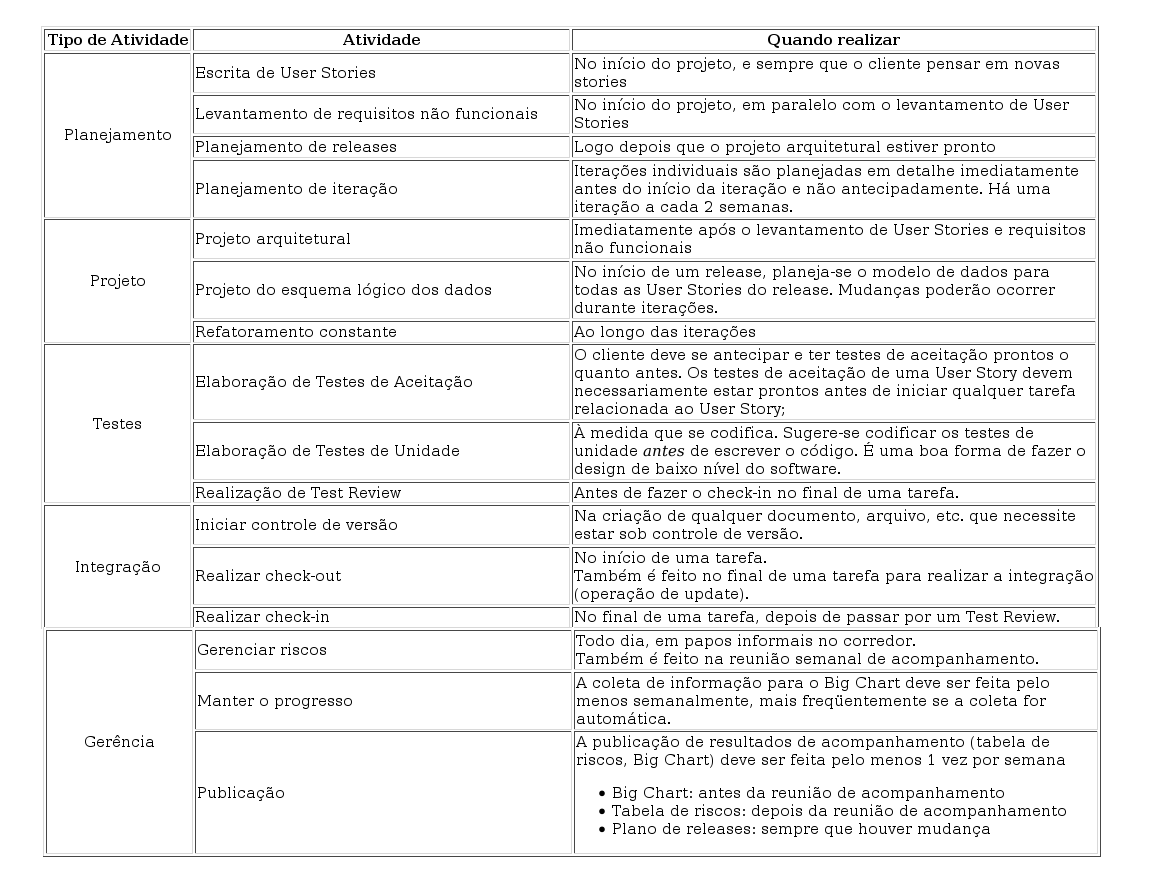
\includegraphics[height = 14cm]{tab1.png}
%  \caption{\it Tabela que descreve quando as atividades de XP1 devem ser realizadas.} \label{tab:tab1}
% \end{figure}

\begin{figure}[!h]
 \flushleft
 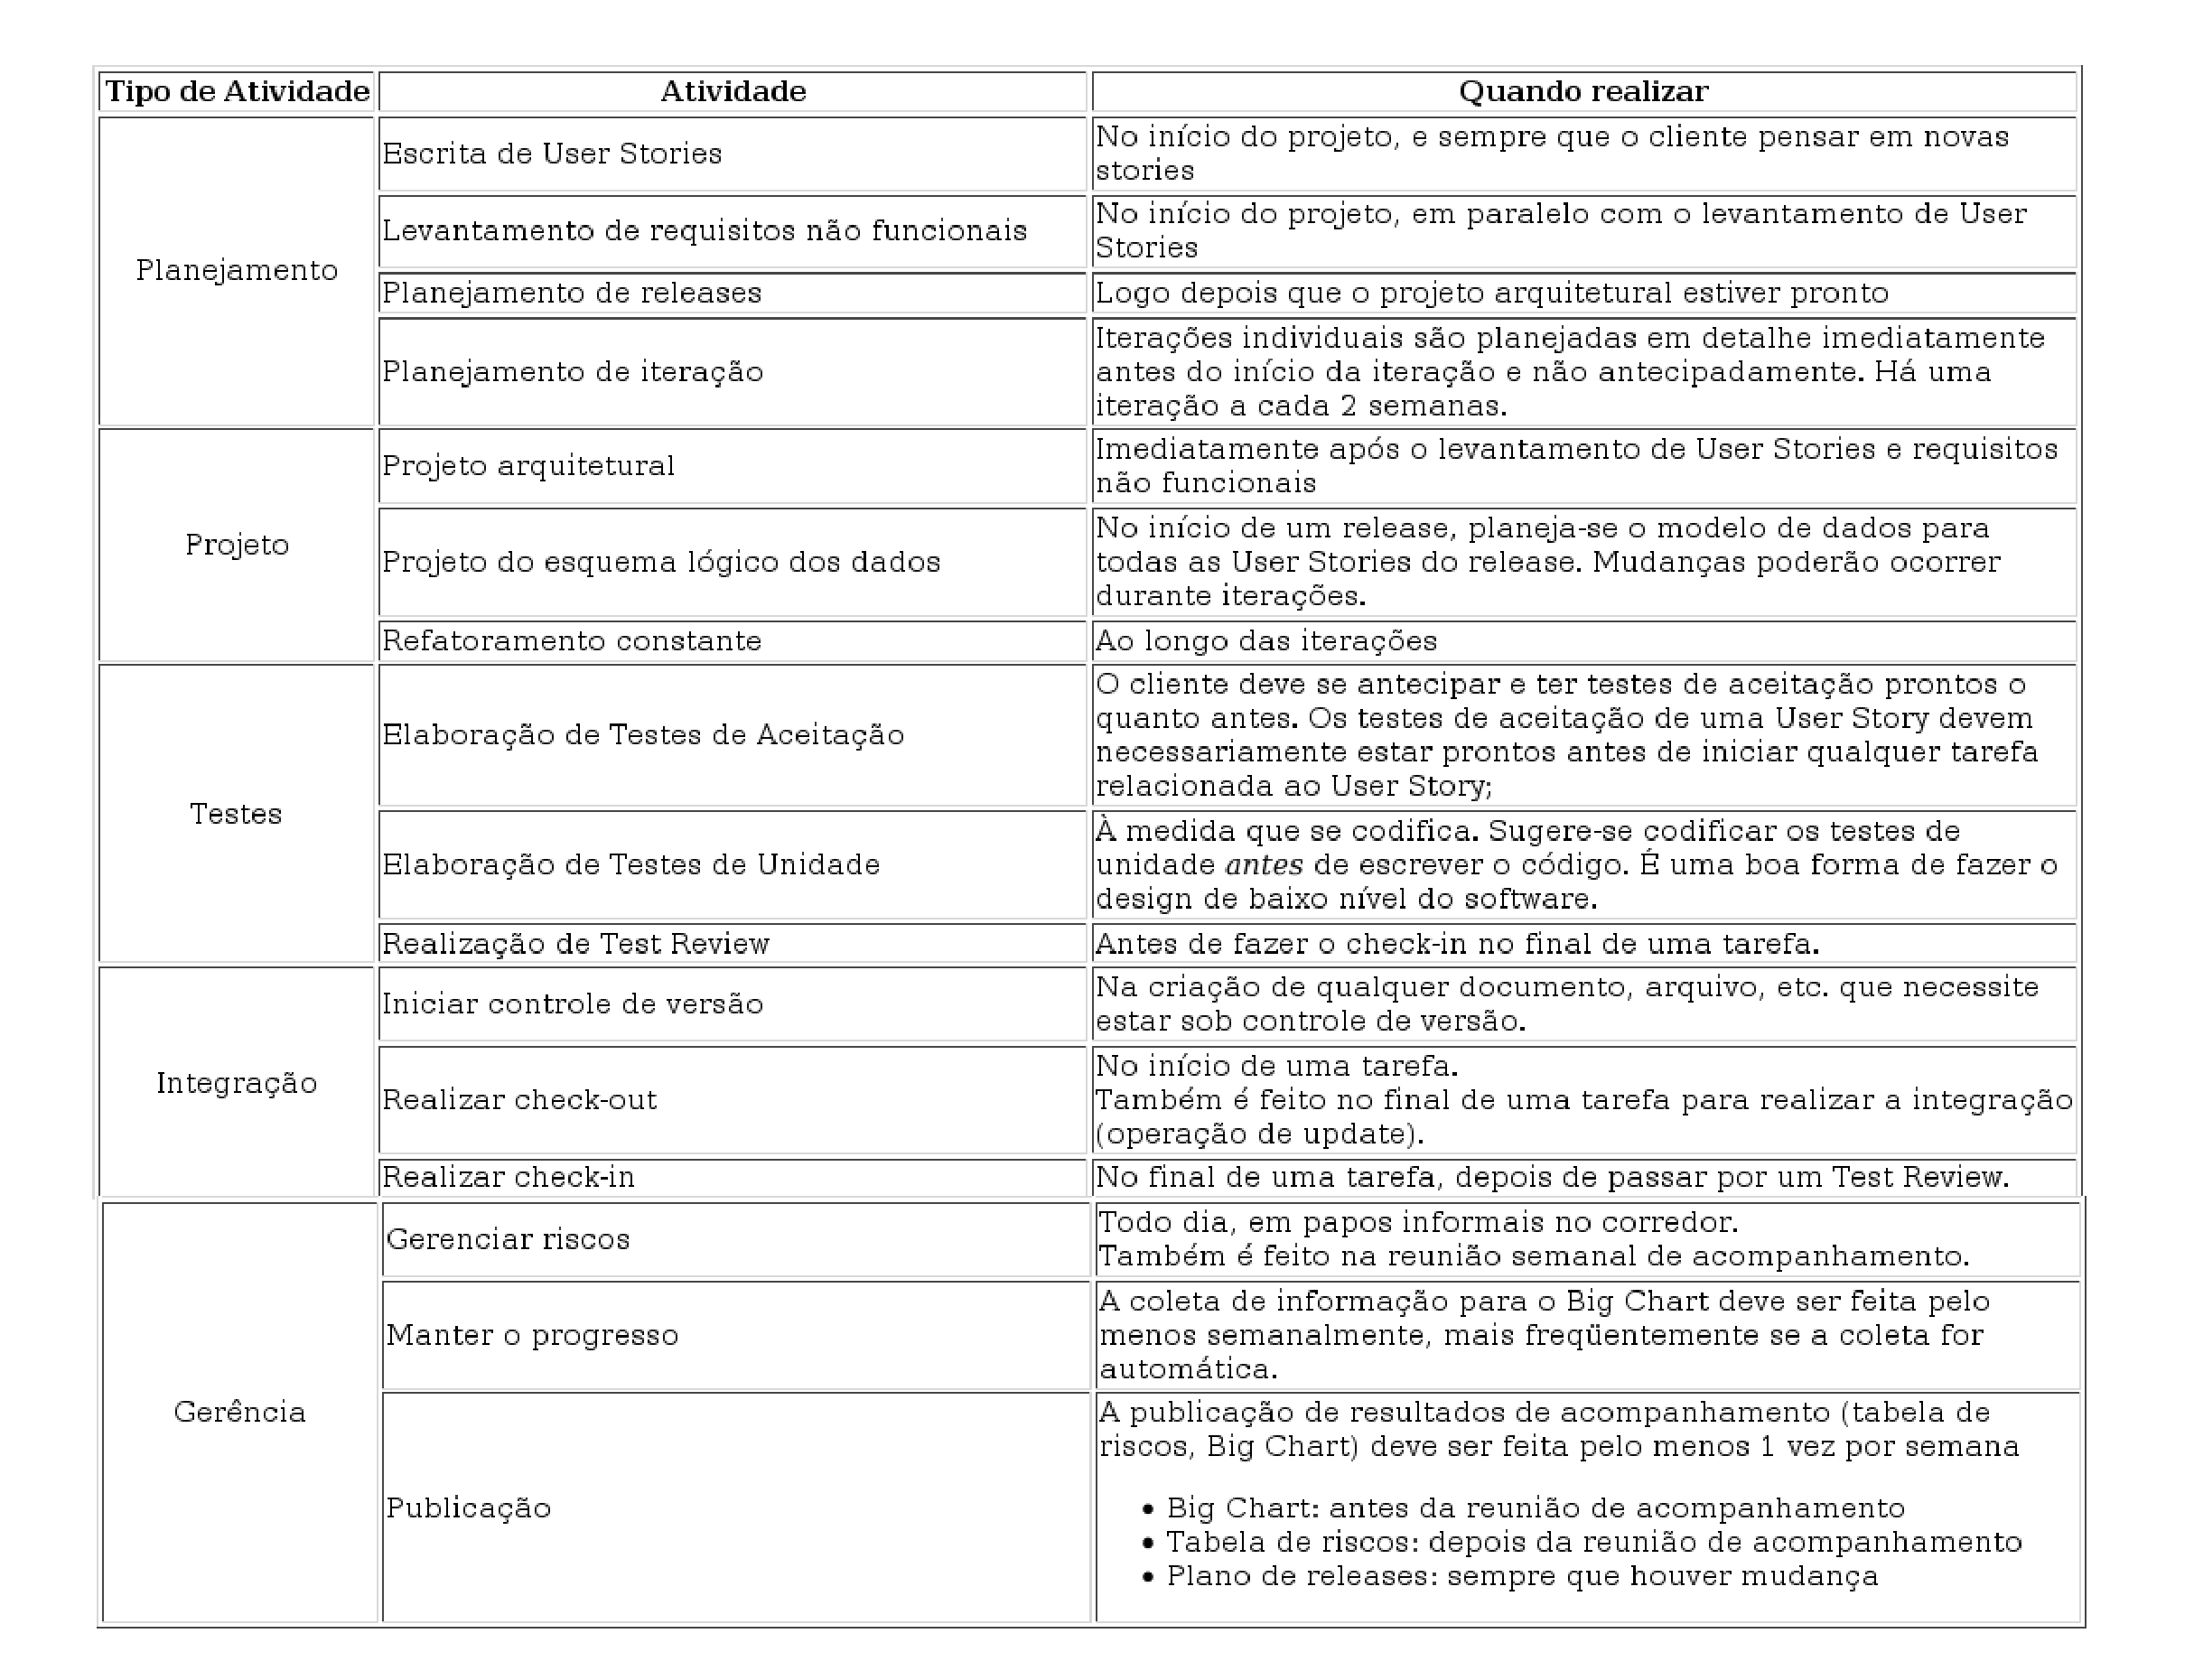
\includegraphics[scale=0.38]{tab1.eps}
 \caption{\it Tabela que descreve quando as atividades de XP1 devem ser realizadas.} \label{tab:tab1}
\end{figure}

%\begin{table}[h]
% \caption{Tabela que descreve quando as atividades de XP1 devem ser realizadas}
% \centering
% \begin{tabular}{c|l|l}
%  \hline \hline
%  Tipo de Atividade & Atividade & Quando Realizar\\
%  \\[0.5ex]
%  \hline
%  Planejamento & Escrita de User Stories; \cline{1-1}
%  Levantamento de requisitos não funcionais; 
  %Planejamento de releases; Planejamento de iteração 
%  & No início do projeto, e sempre que o cliente pensar em novas stories; \\
  %No início do projeto, em paralelo com o levantamento de User Stories;
  %Logo depois que o projeto arquitetural estiver pronto; 
  %Iterações individuais são planejadas em detalhe imediatamente antes do início da iteração e não antecipadamente;
  %Há uma iteração a cada 2 semanas.\\
%  z & 2
% \end{tabular}
%\end{table}

Instanciando os papéis identificados anteriomente (cliente, desenvolvedor e gerente) no contexto do projeto obtém-se a seguinte classificação: i) o professor Dr. Hyggo O. de Almeida assumiu o papel de cliente; ii) quanto ao papel de gerente, cada um dos integrantes da equipe assumiu a chefia do grupo por um determinado tempo durante o desenvolvimento (aproximadamente um mês cada); e iii) por tratar-se de um número reduzido de pessoal para execução do trabalho, durante o decorrer do projeto todos integrantes foram desenvolvedores/testadores.

Quanto à alocação de atividades (descritas na Tabela \ref{tab:tab1} retirada de \cite{xp1}), houve sempre a preocupação em dividí-las igualitariamente entre os membros da equipe. Para tal, reuniões de acompanhamento foram realizadas semanalmente. Nessas reuniões os membros da equipe procuravam alocar, segundo as habilidades de cada indivíduo, as atividades do modo mais adequado possível. Não havendo acordo, ficava a cargo do gerente da vez impor sua decisão final.

Adaptando as atividades elencadas pelo XP1 ao contexto do projeto percebe-se a seguinte configuração: 
\begin{itemize}
 \item  A atividade de planejamento consumiu bastante tempo ainda na primeira parte da disciplina de Projeto I. Isto deve-se ao fato que esta etapa envolveu uma ampla pesquisa na literatura especializada (e discussões com o cliente) para verificação de quais requisitos, funcionais e não funcionais, deveriam estar presentes no produto final. Com os requisitos já identificados e com as \textit{User Stories} escritas, o próximo passo foi realizar o planejamento das iterações e \textit{releases}. É válido salientar que apesar de todo esse planejamento ter sido realizado durante as primeiras etapa do processo, a cada semana, durante as reuniões de acompanhamento, uma revisão sobre esses artefatos era realizada para garantir que o que se havia planejado realmente estava de acordo com a realidade do problema e da equipe. Portanto, alterações pontuais nos artefatos de planejamento foram realizadas durante todo o processo de desenvolvimento.
 \item A atividade de projeto foi iniciada imediatamente após a conclusão da etapa de planejamento. De posse das \textit{User Stories} e dos requisitos do sistema a equipe em conjunto montou o projeto arquitetural do sistema. O projeto arquitetural decidido foi simplificado, baseado pricipalmente nas ideias de \textit{Model-View-Controller} (MVC), porém atendeu as necessidades ali presentes. Quanto ao esquema lógico, por tratar-se de um projeto que não envolve grandes manipulações de dados, a equipe decidiu por não adotar um banco de dados, e apenas trabalhar com arquivos XML, quando necessário.
 \item Dada a importância que a atividade de testes tem para um bom produto final, a equipe buscou construir suites de teste de qualidade para que estas pudessem localizar rapidamente possíveis deficiências do código. Para tal, logo que as \textit{User Stories} foram escritas os testes de aceitação das mesmas já começaram a ser escritos em sequência. E, seguindo o que indica a metodologia de testes \textit{Test-Driven Development} (TDD) \cite{TDD}, os testes de unidade foram sempre desenvolvidos antes que a codificação fosse realizada. É importante destacar que como o projeto foi proposto por um cliente que não era da área financeira, os testes de aceitação foram escritos pelos desenvolvedores junto ao mesmo a partir de materiais de exercícios financeiros encontrados na Internet, incluindo os manuais da HP-12C \cite{man1} \cite{man2} \cite{man3} \cite{man4} e o material de matemática financeira do professor Adail Marcos Lima Da Silva \cite{adail}, sempre comparando os resultados obtidos com os da HP-12C real. Outro ponto importante é que existiu sempre a preocupação de que pessoas diferentes escrevessem e revisassem os testes, procurando, assim, garantir uma maior credibilidade.

 \item A atividade de integração foi uma preocupação constante da equipe desde a fase de planejamento. Para que não ocorressem divergências ou inconsistências de conteúdo, surgiu a preocupação de criar um controle de versões tanto para a biblioteca financeira quanto para a calculadora \textit{Pyfinancial}, para tal fez-se uso das já muito conhecidas ferramentas de controle de versões SVN \cite{SVN} e Garage \cite{garage}. O SVN foi utilizado para controle apenas da biblioteca financeira, dado que ela é um software livre e \textit{open-source}, de modo a ganhar visibilidade para a mesma entre desenvolvedores Python, ao passo que o Garage foi utilizado para a calculadora financeira procurando dar-lhe visibilidade junto a plataforma Maemo. Com isso, manteve-se um controle sistematizado do código, bem como dos artefatos de planejamento.

 \item Quanto à realização de \textit{Reviews}, sempre foi realizado um tempo após a escrita dos testes e do código funcional para a revisão da qualidade dos testes escritos (verificando novamente os resultados com a calculadora, observando coerência e cobertura dos mesmos, etc.), bem como para realizar algum refatoramento que se mostrasse necessário de maneira imediata. Embora tenha-se procurado organizar o design de maneira flexível, percebeu-se no decorrer do projeto que alguns pontos poderiam sofrer um refatoramento maior. Essa necessidade possivelmente está relacionada com o fato de não ter sido alocado desde o início um tempo maior para \textit{Code} e \textit{Design Review}.

 \item Por fim, como já dito anteriormente, a atividade de gerência foi revesada entre os membros da equipe. Cada um atuou como gerente por um determinado período de tempo durante a realização do projeto. Ao gerente coube entender as mudanças discutidas durante as reuniões de acompanhamento e refleti-las tanto nos artefatos de planejamento (\textit{User Stories}, requisitos, projeto arquitetural etc), quanto nos artefatos de gerência (\textit{Big-Chart}, a tabela de riscos  e o plano de \textit{releases} etc). Essa atividade foi realizada sempre em paralelo com o desenvolvimento da aplicação, aproximadamente uma vez a cada semana.
 
\end{itemize}

Para garantir que as atividades fossem realizadas da forma mais adequada possível uma infra-estrutura foi montada a fim de melhorar a organização e consequentemente a qualidade do código produzido. Dentre os elementos presentes nessa infra-estrutura podemos destacar:

\begin{itemize}
 \item \textbf{Eclipse} \cite{eclipse}. IDE de desenvolvimento.
 \item \textbf{PyDev} \cite{pydev}. \textit{Plug-in} para desenvolvimento em Python.
 \item \textbf{PyUnit} \cite{pyunit}. \textit{Framework} para desenvolvimento de testes de unidade.
 \item \textbf{PyEasyAccept} \cite{pyeasyaccept}. \textit{Framework} para desenvolvimento de testes de aceitação.
 \item \textbf{SVN e Garage SVN} \cite{SVN}\cite{garage}. Ferramentas para controle de versões.
\end{itemize}
